\begin{frame}{Componentes Adapter y ListView en Android}
\textbf{¿Qué es ListView?}

\begin{itemize}
    \item Es un componente de interfaz que permite mostrar una lista desplazable de elementos.
    \item Cada elemento puede contener texto, imágenes u otros componentes.
    \item Es útil para mostrar datos en forma de lista vertical.
\end{itemize}

\vspace{0.4cm}

\textbf{¿Qué es un Adapter?}

\begin{itemize}
    \item Es un intermediario entre los datos y el ListView.
    \item Se encarga de convertir los datos (arreglos, listas, bases de datos) en vistas visuales.
    \item Permite personalizar cómo se muestra cada elemento de la lista.
\end{itemize}

\vspace{0.4cm}

\textbf{Relación entre Adapter y ListView:}
\begin{itemize}
    \item El ListView solicita los datos al Adapter.
    \item El Adapter genera la vista de cada elemento.
\end{itemize}


\end{frame}



\begin{frame}{Componentes Adapter y ListView en Android}
\textbf{¿Qué es ListView?}

\begin{itemize}
    \item Es un componente de interfaz que permite mostrar una lista desplazable de elementos.
    \item Cada elemento puede contener texto, imágenes u otros componentes.
    \item Es útil para mostrar datos en forma de lista vertical.
\end{itemize}

\vspace{0.4cm}

\textbf{¿Qué es un Adapter?}

\begin{itemize}
    \item Es un intermediario entre los datos y el ListView.
    \item Se encarga de convertir los datos (arreglos, listas, bases de datos) en vistas visuales.
    \item Permite personalizar cómo se muestra cada elemento de la lista.
\end{itemize}

\vspace{0.4cm}

\textbf{Relación entre Adapter y ListView:}
\begin{itemize}
    \item El ListView solicita los datos al Adapter.
    \item El Adapter genera la vista de cada elemento.
\end{itemize}


\end{frame}



\begin{frame}[fragile]
\frametitle{Demo 06: Agregar un ListView}
\begin{columns}
\column{0.80\linewidth}
Del Repositorio Github:
\begin{itemize}
\item Copiar el archivo MainActivity\_Demo06.java (dentro del Folder códigosJAVA) al mismo directorio donde esta el MainActivity.java
\item Copiar el archivo activity\_main\_demo06.xml (dentro del Folder Carpeta\_layout) al mismo directorio donde esta el activity\_main.xml
%\item Copiar los archivos \textit{cgup.jpg} y \textit{logo\_upv\_2019.png} localizados dentro de la folder \textit{Carpeta\_drawable} en el directorio \textit{res/drawable} del proyecto de AS.
\item Modificar en el archivo AndroidManifest.xml la cadena \textit{.MainActivity\_Demo05} por \textit{.MainActivity\_Demo06}
\end{itemize}

\begin{block}{Demo \#06}
Muestra una App con un ListView. El usuario agregar elementos al presionar el boton superior.    
\end{block}


\column{0.20\linewidth}

\begin{center}
 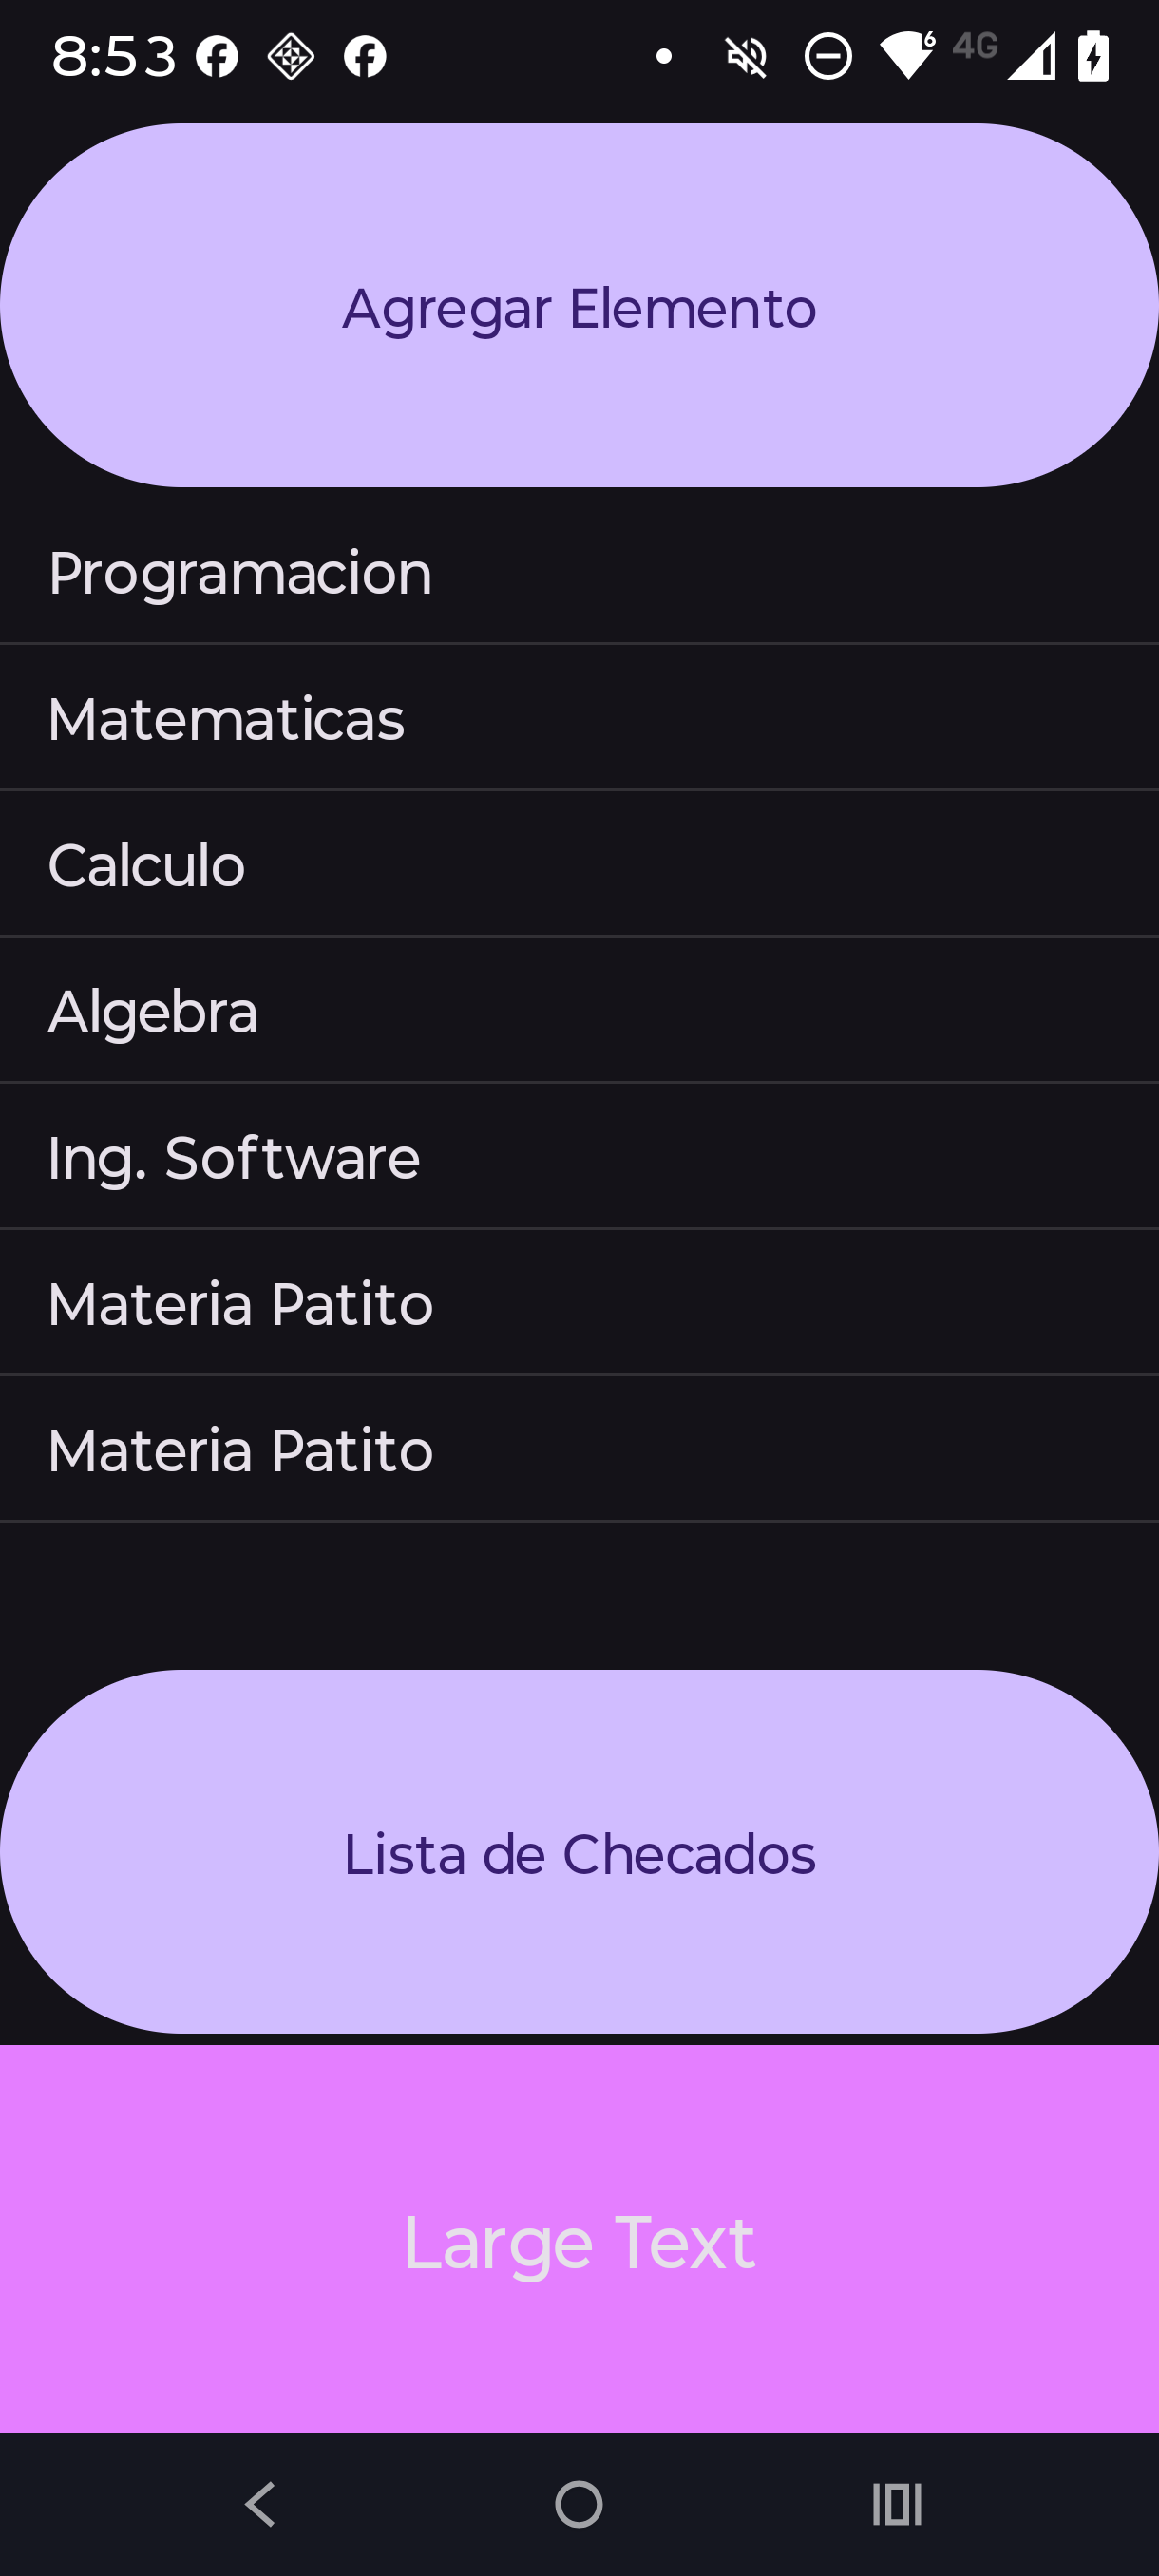
\includegraphics[width=0.98\textwidth]{02_TallerCBTis/figs/Demo06}
\end{center}

\end{columns}

\end{frame}

